%
% lochkamera.tex
%
% (c) 2018 Prof Dr Andreas Müller, Hochschule Rapperswil
%
\documentclass[tikz,12pt]{standalone}
\usepackage{times}
\usepackage{amsmath}
\usepackage{txfonts}
\usepackage[utf8]{inputenc}
\usepackage{graphics}
\usepackage{color}
\usepackage{pifont}
\usetikzlibrary{arrows,intersections,math,calc}
\begin{document}

\def\punkt#1{
        \fill[color=white] #1 circle[radius=0.08];
        \draw #1 circle[radius=0.08];
}

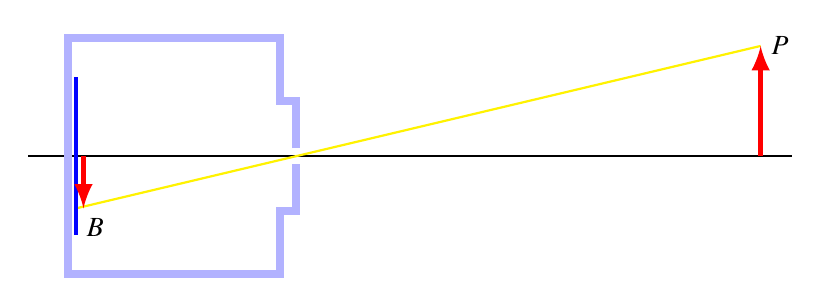
\begin{tikzpicture}[>=latex,thick]

\tikzmath{
	real	\r;
	\r = 2.5;
	real	\w, \v;
	\w = atan(0.7/2.5);
	\v = atan(0.7/5);
	real	\x, \y;
	real	\a, \b, \c;
	\x = 5.8;
	\y = 1.4;
	\c = -0.1;
	\a = -2.9;
	\b = \y * (\a - \c) / (\x - \c);
}

\draw[line width=0.5pt] (-3.5,0)--(6.2,0);

%\fill[color=gray] (0,-0.7) arc ({-\w}:{\w}:{\r})
%	--(-0.1,0.7) arc ({180-\w}:{180+\w}:{\r})--cycle;
%
%\fill[color=gray] (-0.12,0.7) arc ({180-\w}:{180+\w}:{\r})
%	--(-0.3,-0.7) arc ({180+\v}:{180-\v}:{2*\r})--cycle;

%\foreach \t in{-0.6,-0.4,...,0.61}{
\def\t{0}
\draw[color=yellow] ({\x},{\y})--({\c},{\t})--({\a},{\b});
%}

\draw[color=blue!30,line width=3pt]
	({\c},0.1)--({\c},0.7)--
	(-0.3,0.7)--(-0.3,1.5)--(-3,1.5)
		--(-3,-1.5)--(-0.3,-1.5)--(-0.3,-0.7)
		--({\c},-0.7)--({\c},-0.1);

\draw[color=blue,line width=1.5pt] (-2.9,-1.0)--(-2.9,1.0);

\draw[->,color=red,line width=2pt] ({\x},0)--({\x},{\y});
\draw[->,color=red,line width=2pt] ({\a+0.1},0)--({\a+0.1},{\b});

\node at ({\x},{\y}) [right] {$P$};
\node at ({\a},{\b}) [below right] {$B$};

\end{tikzpicture}

\end{document}

